% Chapter Template

\chapter{Introduction} % Main chapter title

\label{Chapter1} % Change X to a consecutive number; for referencing this chapter elsewhere, use \ref{ChapterX}

%-------------------------------------------------------------------------------------
%	INTRODUCTION
%-------------------------------------------------------------------------------------

Oxidation and reduction (redox) reactions play a vital role in biology. These reactions are characterized by a flow of electrons between chemical species. The species gaining electrons is said to have been oxidized, while the species losing electrons is said to have been reduced. Redox reactions are involved in many vital processes such as cellular respiration, \todo{other processes}.

Many chemical species in the cell may exist in either an oxidized or reduced form. These \textit{redox couples} play central roles in a variety of cellular processes. The NAD\textsuperscript{{+}}/NADH couple, for example, shuttles high energy electrons wrought from the oxidation of sugars in the citric acid cycle to the proton pumps in the electron transport chain. The healthy cell actively maintains a steady-state disequilibrium of these redox couples. The overall state of this network of redox couples is called the \textit{redox state}. The impaired ability of the cell to regulate its redox state is termed \textit{oxidative stress} and is associated with a number of diseases such as cancer, various neurological disorders, and aging. Quantifying the redox state in live cells allows a deeper understanding of the regulatory mechanisms that mediate these processes.

%-------------------------------------------------------------------------------------
%	SECTION 1
%-------------------------------------------------------------------------------------
\section{Fluorescent biomarkers enable real-time quantification of cytosolic protein oxidation} \label{fluorescenceIntro}
In a previous paper, our lab demonstrated the use of the redox-sensitive fluorescent protein roGFP to quantify the cytosolic redox state in the pharyngeal muscle of \textit{C. elegans} in real-time. The use of these biomarkers is leading to quantitative and mathematical models of the genetics and dynamics of intracellular and organismal-level redox signaling.

The methodology relies on the dual emission spectra of the oxidized and reduced form of roGFP. By taking the ratio of emission intensity when excited at different wavelengths, we can use the Nernst equation to estimate the cellular redox state.

The quantification requires two images be taken of each pharynx --- one at 410nm and another at 470nm. By dividing the brightness of the images pixel-by-pixel we can estimate the redox state at each position in two dimensions (Figure \ref{fig:ratioImageToE}).

\begin{figure}[ht]
    \centering
    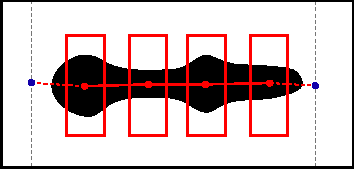
\includegraphics[scale=1.5]{Figures/rendered_files/old_midline_algorithm}
    \decoRule
    \caption[Ratios of images to redox state]{}
    \label{fig:ratioImageToE}
\end{figure}

\todo[inline]{replace fig this with the 410nm / 470nm => E}

Due to the cellular architecture of the pharynx, almost all of the variation in redox state follows the posterior-anterior axis. Thus, we can model the pharynx 1-dimensionally as the redox state along its posterior-anterior axis without losing significant information. Computationally, this is achieved by (1) estimating the centerline of the pharynx then (2) measuring the intensity of the images under this estimated centerline.

As will be discussed, a fundamental limitation of this analysis arises when the animal moves in the time between capturing the first and second frame in the pair of images required for each animal. The aim of this thesis project was to improve the methods by which these centerline measurements were gathered and analyzed so as to reduce experimenter input and minimize errors introduced by this inter-frame movement. 

%-------------------------------------------------------------------------------------
%	SECTION 2
%-------------------------------------------------------------------------------------
\section{Limitations of current pipeline} \label{limitations}
\subsection{Inter-frame movement results in measurement error} \label{limitationMovement}

The pharynx is the feeding muscle of the animal. It contracts along its anterior-posterior axis, functioning as a pump to bring in food. Animals are paralyzed prior to imaging with a 1mM solution of the actyl choline agonist levamisole. Even so, the pharyngeal muscle occasionally contracts. 

This contraction poses a problem for analysis. Ordinarily, dividing intensities pixel-by-pixel is appropriate because the mapping between image space and physical space remains consistent between pairs of images. If the animal moves, however, a new mapping must be constructed for each image. To understand  why, consider Figure \ref{fig:ContractionsCartoon}.

\begin{figure}[ht]
    \centering
    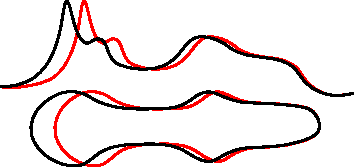
\includegraphics{Figures/rendered_files/contraction_cartoon}
    \decoRule
    \caption[Pharyngeal contractions lead to boundary issues]{A cartoon shows how pharyngeal contractions lead to measurement boundary issues.}
    \label{fig:ContractionsCartoon}
\end{figure}

On the bottom we see the outline of the pharynx in each frame. The pharynx has contracted in one frame (red) and is elongated in the other (black). When the intensities along the posterior-anterior axis are plotted above, it is clear that the contraction has lead to unwanted compression of the intensity profile.

Another common mode of interframe movement is represented similarly in Figure \ref{fig:DorsalVentralCartoon}. This is movement of the tip of the pharynx dorsal-ventrally. Dorsal-ventral tip movements result in a loss of information about the tip in one frame, as depicted in red.

\begin{figure}[ht]
    \centering
    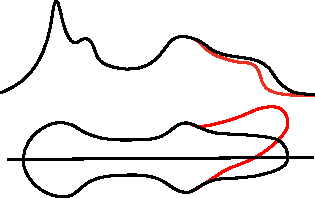
\includegraphics{Figures/rendered_files/dorsalventral_cartoon}
    \decoRule
    \caption[Dorsal ventral movement of the tip of a pharynx]{A cartoon shows dorsal ventral movement in the tip of the pharynx and the resultant intensity profiles measuring under the single centerline.}
    \label{fig:DorsalVentralCartoon}
\end{figure}

The current method for dealing with these problems is to visually screen the ratio images for images with a highly textured appearence, as shown in figure \ref{fig:HighMovement}. These animals are then excluded from analysis. This visual screening is a time-intensive process, requires training, and is subject to experimenter error and bias.

\begin{figure}[ht]
    \centering
    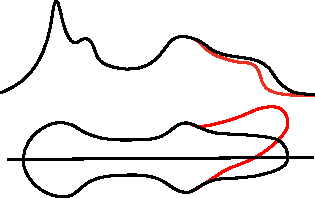
\includegraphics{Figures/rendered_files/dorsalventral_cartoon}
    \decoRule
    \caption[Dorsal ventral movement of the tip of a pharynx]{A cartoon shows dorsal ventral movement in the tip of the pharynx and the resultant intensity profiles measuring under the single centerline.}
    \label{fig:HighMovement}
\end{figure}

\subsection{Segmentation and centerline estimation sometimes require manual input}\label{limitationManual}

As noted, the visual screen for inter-frame movement is a manual step. Two other processes in the current pipeline also require manual supervision. The first is segmentation. Segmentation is the process by which pixels corresponding to objects in an image are given salient labels. In our case, the task is to separate the pharynx from everything else (Figure \ref{fig:SegmentationExample}). 

\begin{figure}[ht]
    \centering
    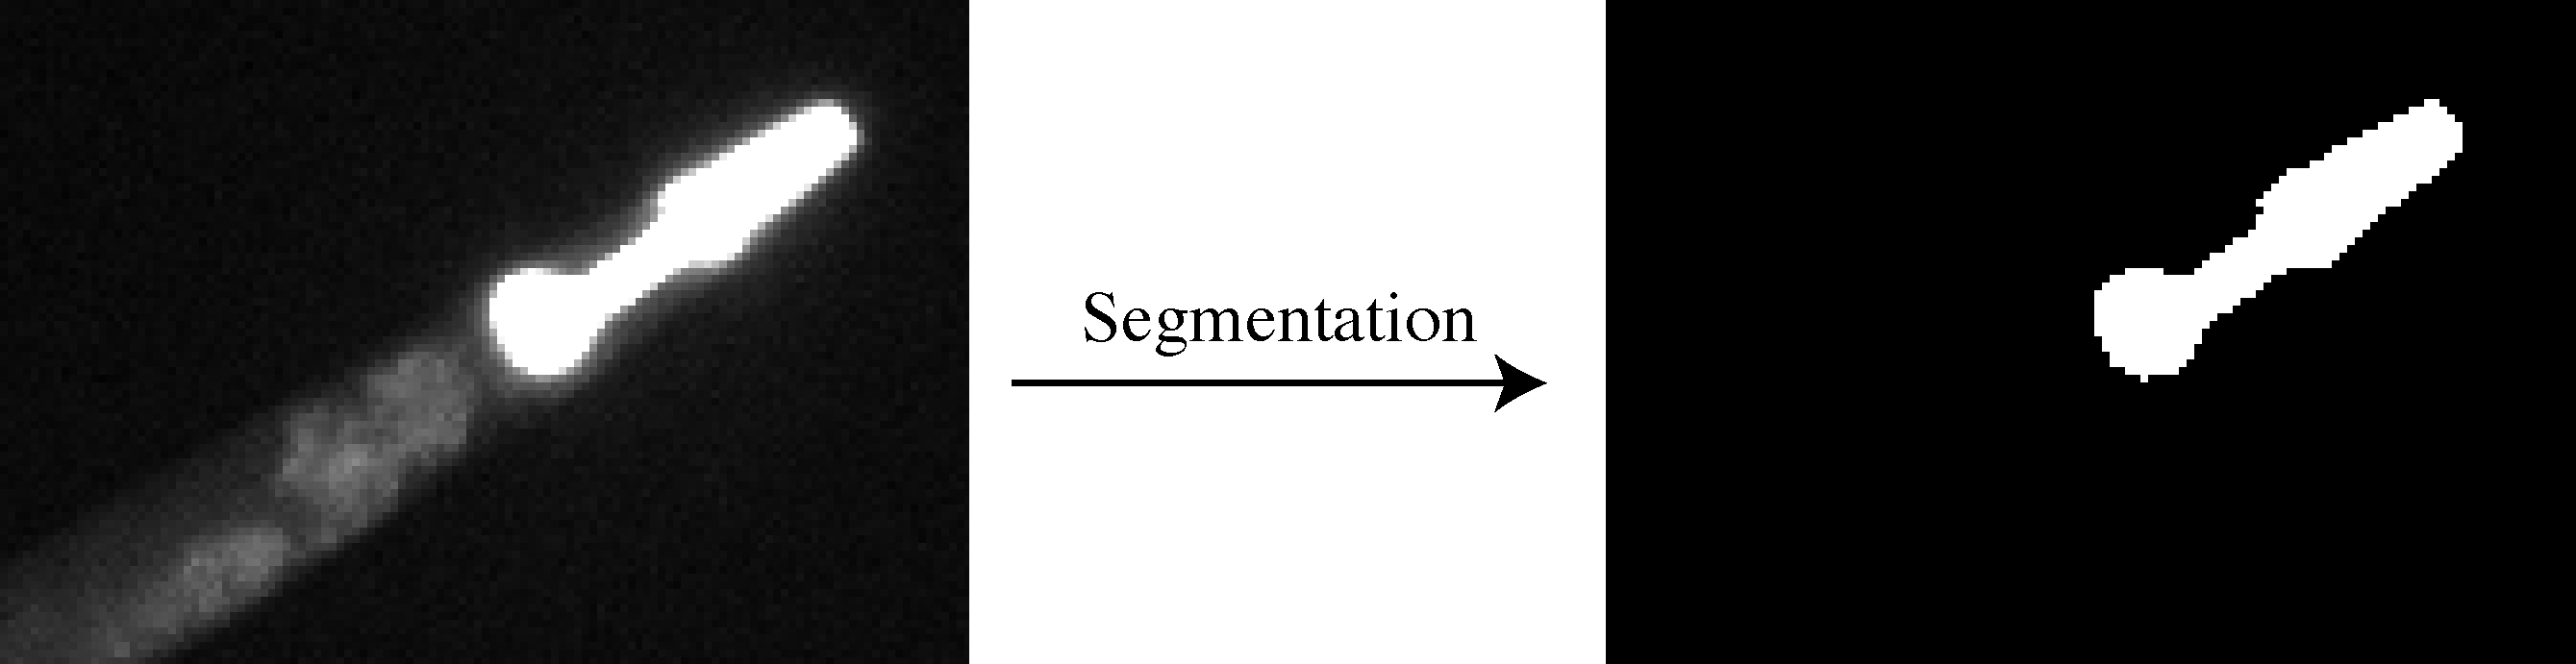
\includegraphics[scale=.25]{Figures/rendered_files/segmentation_description}
    \decoRule
    \caption[The goal of segmentation]{The goal of segmentation. On the left, the original image showing fluorescence of roGFP in the pharynx and autofluorescence in the gut. On the right, a binary image consiting of value \texttt{1} in the pixels with a pharynx and value \texttt{0} elsewhere.}
    \label{fig:SegmentationExample}
\end{figure}

Because the transgenic animals express roGFP with pharynx-specific promoters, the task is usually straightforward. However, the intenstine of \textit{C. elegans} autofluoresces in response to the wavelengths of light that we use. This poses a problem for the static thresholding algorithm currently used to segment the pharynx. This algorithm assigns any value greater than a threshold the value \texttt{1} and those below the threshold \texttt{0}. Static thresholds works well when the distribution of brightness is different for each class of object in the image, but this is not the case when the intestine autofluoresces resulting in ill-formed segmentation masks (Figure \ref{fig:SegmentationNaive}).

\begin{figure}[ht]
    \centering
    
\includegraphics[scale=.25]{Figures/rendered_files/segmentation_naive}
    \decoRule
    \caption[The problem with static thresholding]{The problem with static thresholding. This image must be manually corrected.}
    \label{fig:SegmentationNaive}
\end{figure}

\section{Aims}
This thesis aims to address the limitations of the current analysis pipeline described in \ref{limitationMovement} and \ref{limitationManual}. To achieve this, a new pipeline was written in MATLAB to process and analyze these images end-to-end with little to no necessary manual input. The improved pipeline decreases the time required to analyze this data, standardizes the analysis, reduces human error, and mitigates movement-induced error.